% This must be in the first 5 lines to tell arXiv to use pdfLaTeX, which is strongly recommended.
\pdfoutput=1
% In particular, the hyperref package requires pdfLaTeX in order to break URLs across lines.

\documentclass[11pt]{article}

% Remove the "review" option to generate the final version.
\usepackage[]{acl}

% Standard package includes
\usepackage{times}
\usepackage{latexsym}
\usepackage{graphicx}

% For proper rendering and hyphenation of words containing Latin characters (including in bib files)
\usepackage[T1]{fontenc}
% For Vietnamese characters
% \usepackage[T5]{fontenc}
% See https://www.latex-project.org/help/documentation/encguide.pdf for other character sets

% This assumes your files are encoded as UTF8
\usepackage[utf8]{inputenc}

% This is not strictly necessary, and may be commented out,
% but it will improve the layout of the manuscript,
% and will typically save some space.
\usepackage{microtype}

% If the title and author information does not fit in the area allocated, uncomment the following
%
%\setlength\titlebox{<dim>}
%
% and set <dim> to something 5cm or larger.

\title{Crossword Answer PoS Prediction with Contextual Embeddings}

\author{
  Henry Pick \\
  Harvey Mudd College \\
  \texttt{hpick@hmc.edu} \\\And
  Miles Christensen \\
  Harvey Mudd College \\
  \texttt{mchristensen@hmc.edu}
 }

\begin{document}
\maketitle

\begin{abstract}
    In this paper, we implement a morphological classifier similar to those found in multiple common crossword solving systems. This task involves assigning part of speech tags to crossword answers based only on the text of the clue. We demonstrate that using the contextual embeddings of a pre-trained BERT model for sequence classification is a viable method for this classification task.
\end{abstract}

\section{Introduction}
Crossword solving as a problem in NLP has been studied for years. The first system designed to programmatically solve crosswords was Proverb \cite{Keim99-PROVERB, Littman02-AProbabilistic}, and two more modern state-of-the-art solvers are WebCrow \cite{Angelini05-Webcrow} and Dr. Fill \cite{Ginsberg11-DrFill}. While most of these systems have long been in development, there is no agreed-upon best architecture for programmatic crossword solving. Furthermore, all of these systems are quite complex, consisting of many stages of processing and several tiers of abstraction. These reasons all make the component-wise performance of each system opaque and thus make it difficult for a reader of one of these works to make objective evaluations of such systems.

Our work focuses on a critical processing stage in WebCrow's architecture called morphological filtering. At this stage, potential candidate answers are ranked or discarded based on certain morphological characteristics that the filter infers from the clue. If this filter performs well, then the candidate lists are small and accurate, giving the constraint problem solver a significantly easier puzzle to solve. Because there is no documented performance for this morphological filter, we have no idea if we could do better with cutting-edge NLP tools. In this work, we will design our own morphological filter and evaluate it against metrics that indicate how it might perform in an actual crossword solving system. We will not be developing a full-fledged crossword solver, as this is much too large a task to accomplish in a single research paper and it involves a large amount of focus outside the field of NLP.
\section{Related Work}
\subsection{Crossword solving}
Proverb and WebCrow adopt a modular approach for generating candidate answers: clues are fed to multiple different modules that each produce their own set of candidates, which are then merged to provide a full list of candidates for each clue. With these candidate answers, the task of filling the crossword grid can then be formalized as a probabilistic constraint satisfaction problem \cite{Shazeer99-Solving}. In comparison to Dr. Fill and WebCrow, Dr. Fill excels in optimizing solutions to this constraint satisfaction problem with various heuristics and post-processing algorithms. This, however, is outside the scope of our work, and we will focus primarily on the modules of Proverb ad WebCrow.

Many of Proverb's modules rely heavily on a crossword database (CWDB) of over 250,000 unique clue-answer pairs, finding exact matches, partial matches, or measuring the co-occurrence of words in clues and answers. Other modules are domain-specific (such as \verb.Movies. or \verb.Geography.) and query online sources (such as \verb,www.imdb.com, or the Getty Information Institute) to generate candidate answers. WebCrow also has a similar (but significantly smaller) CWDB, but it does not have domain-specific modules; most of its candidate generation is instead performed by a generic web search module. This module reformulates the clue into multiple search engine queries, downloads the resulting documents, then extracts and filters all words in these documents to find appropriate candidates.

\subsection{Morphological filtering}
Both WebCrow and Dr. Fill use filtering techniques to remove unlikely candidates from ranking lists as they are being fetched from a knowledge databases. WebCrow's web search module, for example, uses a morphological filter, a scoring function that ranks words according to their morphological category. The filter first uses TreeTagger \cite{Schmid95-Improvements} to generate a part-of-speech (PoS) tag probability vector for each word in the clue, and then uses these vectors along with other features to classify the clue as a whole using a multi-class Kernel-based Vector Machine \cite{Tsochantaridis04-Support}. The classifier uses features that are present only in the clue and not in the crossword constraint (ie. number of words in the clue, length of the target answer, number of capital letters in the clue). Dr. Fill similarly recognizes that the clue and answer must follow the same morphological constraints, satisfying what is referred to as the ``substitution test''. For example, a clue for the answer \verb.SPAS. is ``Places for mani-pedis''; because the clue is plural, the answer must be as well, so they can be substituted for one another in the context of a sentence.

\subsection{Multi-Class Support Vector Machines}
WebCrow's morphological filter uses a multi-class kernel-based support vector machine. At a high level, this is just an SVM that is able to output multi-class predictions. The ``kernel-based'' part of this name means that the SVM uses a function that maps the inputs into a higher dimensional feature space, allowing the model to create nonlinear boundaries in its prediction space.

The kernel based SVM in WebCrow classifies a list of features including the length of the target, the number of words in the clue, the number of capital letters in the clue, and the probability tag vectors for each word in the clue. Note that these features are all simple and can be readily extracted from each example without using sophisticated pretrained models such as one used for vector embedding. This means that there is a potentially large amount of information being discarded when predicting morphological characteristics of the answer. However, the fact that WebCrow chooses to use this method suggests that it is still advantageous to the morphological filter's performance.

Since WebCrow's initial publication in 2005, there have been significant advances in developing word embedding models that have outperformed traditional feature classifiers in most instances of natural language classification \cite{Mikolov13-word2vec}. One might wonder how a embedding model trained on the raw clues might perform relative to these simpler feature classifiers used by most crossword solvers. In this project, we seek to answer this question by training a BERT contextual embedding model on our own training data. No evaluation metrics for WebCrows kernel-based SVM exist, so we will use our own judgement to determine whether or not our results create a feasible alternative.
\section{Methods}
\subsection{Dataset}
The dataset we will be using is a public dataset at \verb,xd.saul.pw,. It is a set of over 6,000,000 published crossword clue-answer pairs. Each pair has the clue, the answer, the publisher, and the year in which the puzzle was published. Because the dataset was developed independently for a personal project, there is no research paper describing it, but it is provided for public use under the MIT License.
\subsection{PoS Tagging Training Data}
\label{sec:training_data}
A morphological characteristic of interest is the answer's part of speech, which is usually unambiguous to a human inspection and in some cases can be inferred from a PoS tagger. The dataset of answer/clue pairs currently contains no PoS tags and is too large to manually tag in its entirety, meaning our first approach was to create a rough tagset using a automatic PoS tagger. We accomplished this through the standard SpaCy language model tagger on the Penn Treebank Tagset \cite{Marcus93-penntreebank}. Automatic tagging poses a challenge because it only infers the PoS tag from answer word itself without considering the clue in context. Inevitably, many answers will not have one dominant PoS prediction, or will have a blatantly incorrect inference. After inspecting the output of the automatic tagger that we created, we determined it necessary to tag a small subset of the answers manually. In this, we reviewed over 2,500 samples from a random shuffling of the dataset and amended the PoS tags where the automatic tagger had inferred incorrectly. The counts of PoS labels in this dataset are important as they may affect how our model trains. We have recorded this in \ref{tab:pos_frequencies}.
\begin{table}[ht]
    \centering
    \begin{tabular}{c|ccccc}
         & NN & NNP & VB & NNS & JJ \\
         \hline
        Count & 812 & 651 & 300 & 270 & 203\\
        \\
        & FW & VBZ & VBD & RB & IN \\
        \hline
        Count & 65 & 62 & 51 & 46 & 25\\
        \\
        & UH & VBN & NNPS & JJR &\\
        \hline
        Count & 23 & 17 & 11 & 10 &
    \end{tabular}
    \caption{Counts of PTB PoS tags in manually tagged dataset. Remaining counts below 10 are excluded from table.}
    \label{tab:pos_frequencies}
\end{table}

\subsection{Classification with Contextual Embeddings}
Designing a classifier that uses the contextual embeddings from a model like BERT \cite{Devlin18-BERT} to predict PoS of the answer is the main focus of our work. As opposed to the simple feature classifiers, a contextual embedding classifier based on BERT will consider the full or truncated subsection of the semantic expression given in the clue. The training of such a BERT classifier will follows the process of fine-tuning outlined in the original Devlin paper. This simply adds a classification layer to the pre-trained model, training the parameters on the clue-PoS pairs generated in \ref{sec:training_data}.

Among the available tunable BERT models, we chose to work with \texttt{bert-base-cased} provided by the Huggingface NLP project. We chose the cased version because our dataset does have casing in its clues. Compared to some other contextual embedding models like RoBERTa, BERT's performance is certainly less than state-of-the-art. The objective of this project is to assess the viability of a contextual embedding version of a morphological filter. Therefore, we wish to use a model that provides a good baseline for contextual embedding performance as opposed to something more sophisticated.

\subsection{Evaluation Metrics}
Because our task is a multiclass classification problem, we cannot use a simple $F_1$ score. To combine the measured precision and recall from each of these classes, we can use either microaveraging or macroaveraging. In our case, we are assigning exactly one label to each entry so there is no concept of ``true negative''; because of this, the microaveraged precision and recall are the same as accuracy. The macroaveraged $F_1$ score will ignore the relative weights of the classes, which is important to note as our data has a significantly non-uniform distribution of PoS tags. We can also measure and report the $F_1$ score of each class indiviually, allowing us a finer resolution of evaluation that can better inform when the model's output gives valuable predictions. It is conceivable that the morphological filter of WebCrow is used conditionally such that the filter is applied to the candidate list only when certain predictions are made. The $F_1$ table could be used to determine these conditions for our own model and approximate the performance of the filter in a crossword solver.


\section{Results}
We used a random 80/20 split of our manually tagged dataset to train and test out BERT model. Following training, we ran the automatic evaluation metrics and then manually inspected the incorrect predictions to assess the model's weaknesses. Overall, the model's performance on was far better than a base case most-frequent tag classifier which would have a precision and accuracy of $0.39$ and a recall of $1$. In \ref{tab:precisions_recalls}, we observe that the model's performance across the top 5 most frequent tags is fairly uniform, but drops off sharply for less frequent tags as is manifest in the macro average $F_1$ score in \ref{tab:f1_scores}.
\begin{table}[h]
    \centering
    \begin{tabular}{c|ccc}
        class & precision & recall & f1-score\\
        \hline
        NN & 0.67 & 0.81 & 0.73 \\
        NNP & 0.77 & 0.82 & 0.79 \\
        VB & 0.87 & 0.82 & 0.84 \\ 
        NNS & 0.66 & 0.74 & 0.70 \\
        JJ & 0.76 & 0.70 & 0.69
    \end{tabular}
    \caption{Precision and recall evaluations for the model on each of the five most common parts of speech}
    \label{tab:precisions_recalls}
\end{table}
\begin{table}[h]
    \centering
    \begin{tabular}{c|c}
        type & $F_1$ score \\
        \hline
        micro & 0.7223 \\
        macro & 0.3147 \\
        weighted & 0.7023
    \end{tabular}
    \caption{$F_1$ scores computed with different types of averaging}
    \label{tab:f1_scores}
\end{table}
\begin{figure*}[p]
    \centering
    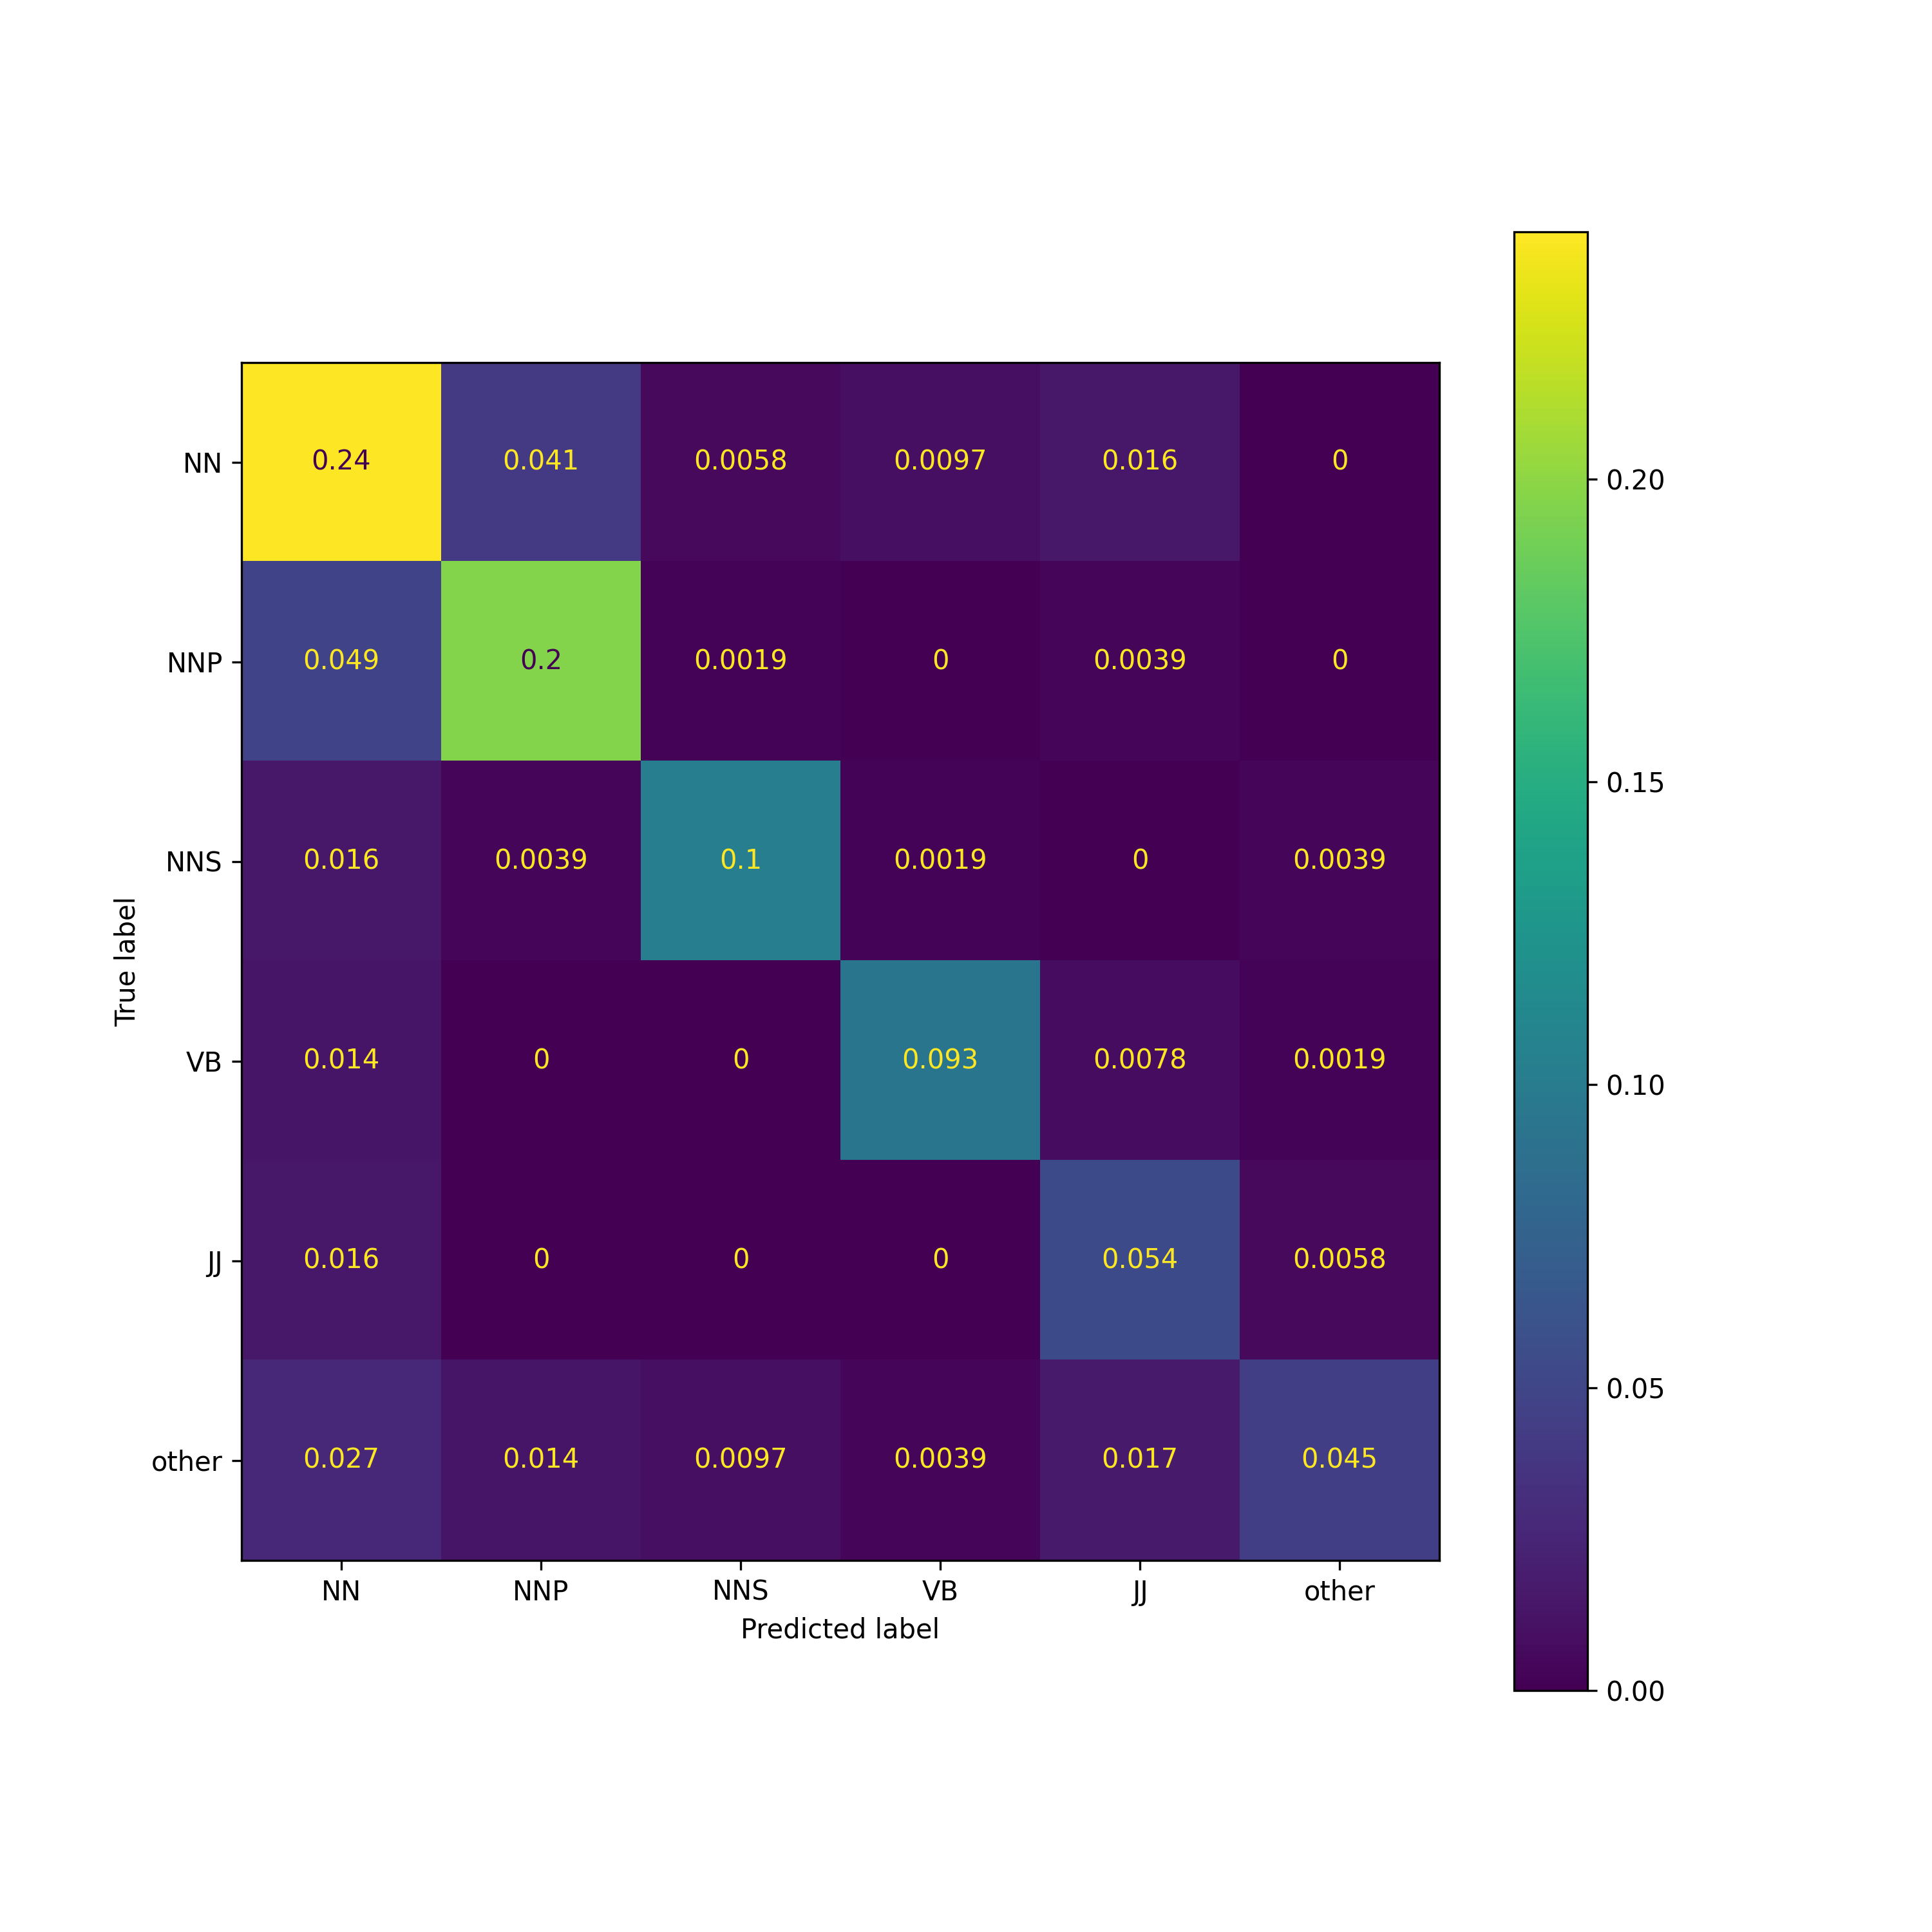
\includegraphics[width=0.9\textwidth]{figures/confusion.png}
    \caption{Confusion matrix shows the contextual embedding model's performance on the four most common PoS labels in the test data. }
    \label{fig:confusion}
\end{figure*}
In \ref{fig:confusion}, this information is represented in a confusion matrix, where correct tag prediction is a clear trend across all 5 of the most common PoS tags. The `other' column accounts for all tags not in this most frequent set.
\subsection{Inaccuracies}
\begin{table*}[t]
    \centering
    \begin{tabular}{c|c|c|c|c}
        category & clue & predicted & actual & answer\\\hline
        wordplay & Aid's partner & NN & VB & ABET \\
        wordplay & Dark or Middle follower & NN & NNS & AGES \\
        proper nouns & A snake charmed her & NN & NNP & EVE \\
        proper nouns & Napoleon Solo, e.g. & NNP & NN & AGENT \\
        ambiguity & Sojourn & VB & NN & TRIP \\
        ambiguity & Lower & JJ & VB & VAIL \\
    \end{tabular}
    \caption{Examples of incorrectly labeled clues.}
    \label{tab:incorrect}
\end{table*}
When our model categorized a clue incorrectly, we found that most often this clue fell into one of three categories: wordplay, proper nouns, and true ambiguity. Examples of these categories are displayed in Table~\ref{tab:incorrect}. 

Clues with wordplay often involve a clue that discusses a word as if the word itself were an entity. Our model generally classifies these clues as common nouns (NN), even though the word itself may be a different part of speech. Without knowledge of common idioms or phrases, recognizing a clue that contains wordplay in this manner would be extremely difficult for a model; it could even be argued that these classifications are not incorrect, because the answer refers to the literal word, not a token in context.

Our model also sometimes incorrectly tags clues for proper nouns (NNP) as common nouns (NN), and vice versa. When a clue involves a person as an example of some category, the model often incorrectly tags the clue with NNP; when a clue involves a cultural reference to a specific person without mentioning other people, the model often incorrectly tags the clue as NN. These incorrect classifications are relatively common, which may be expected as the NN and NNP tags are generally similar in their usage. This type of inaccuracy can be seen clearly in the confusion matrix: the squares corresponding to NN/NNP and NNP/NN are the two highest off-diagonal entries.

Finally, there are some clues that really are ambiguous, and our model guesses just as a human would be required to. This occurs most often when a clue is a single word and the answer is a synonym, but the clue has multiple senses with different parts of speech. We don't expect our model to accurately classify these cases because there is no information to discern between two cases. For a clearer picture of the model's performance overall, it may have helped to remove all single word clues from the dataset and thus remove these truly ambiguous cases.

\section{Conclusion}

In this paper, we described a method to classify crossword clues according to the part of speech of their answer. We used a pre-trained BERT model with  This is a viable strategy for a morphological classifier module, which is a common part of top-end crossword solving systems. 

If this were to be implemented in a full crossword solving system, it is important to be aware of how it would be used. The predicted tags would be used after retrieving candidate answer lists from various modules; however, because our classifier is nowhere near perfect, we cannot simply filter out candidates that do not have a sense that matches the predicted tag. Furthermore, for many tags that are very infrequent, it may be better to simply ignore the results of this classifier because these uncommon tags are susceptible to more errors.

The clearest area for future improvements is simply creating a larger dataset for tagged clue-answer pairs; it may be the case that our model has much room for improvement with more data. This would also help performance on less common tags.

\bibliography{final}
\bibliographystyle{acl_natbib}
\end{document}